\documentclass[../../main.tex]{subfiles}
\begin{document}

\begin{comment}
    Produktbeschreibung des Funktionsmusters
    - Übersichtszeichnungen / Übersichtsmodell
    - Beschreibung der Komponenten
    - Ablaufdiagramme, Blockdiagramme
    - Beschreibung der Funktionalität der einzelnen Blöcke und deren Beziehungen
    - Schnittstellenbeschreibungen
    - Softwaresubsysteme
    - Wichtige Berechnungen (Resultate)
    - Beschreibung von Versuchen und Tests mit Ergebnissen 
\end{comment}

Diese Kapitel beschreibt das Funktionsprinzip des Zuges. Als erstes werden die Mechanischen Komponenten beschrieben. Kapitel \ref{mt_wuerfel} zeigt das Funktionsprinzip der Würfelaufnahmen, Kapitel \ref{mt_Fahrwerk} beinhaltet Angaben zum Fahrwerk und dem Antrieb. \\
Danach wird in Kapitel \ref{et_verbindungen} bis \ref{et_aktoren} die Hardware der Elektronik beschrieben. Anschliessend beschreibt das Kapitel \ref{et_software_tiny} die Software die auf dem Mikrocontroller läuft und die Hardware ansteuert. \\
In Kapitel \ref{aufgabentrennung_pi_tiny} und \ref{interface_pi_tiny} wird die Zusammenarbeit und Kommunikation zwischen dem Mikrocontroller und dem Raspberry Pi beschrieben.
Zum Schluss wird die Software und die dazugehörigen Subsysteme auf dem Raspberry Pi ab Kapitel \ref{it_steuerungssoftware} beschrieben.\\
\\
Abblidung \ref{fig:komponenten_allg} zeigt eine allgemeine Übersicht der einzelnen Komponenten und deren Verbindungen. Genauere Angaben zu den Komponenten und den Verbindungen werden in den Folgenden Kapitel gemacht.\\

\begin{figure}[H]
    \centering
    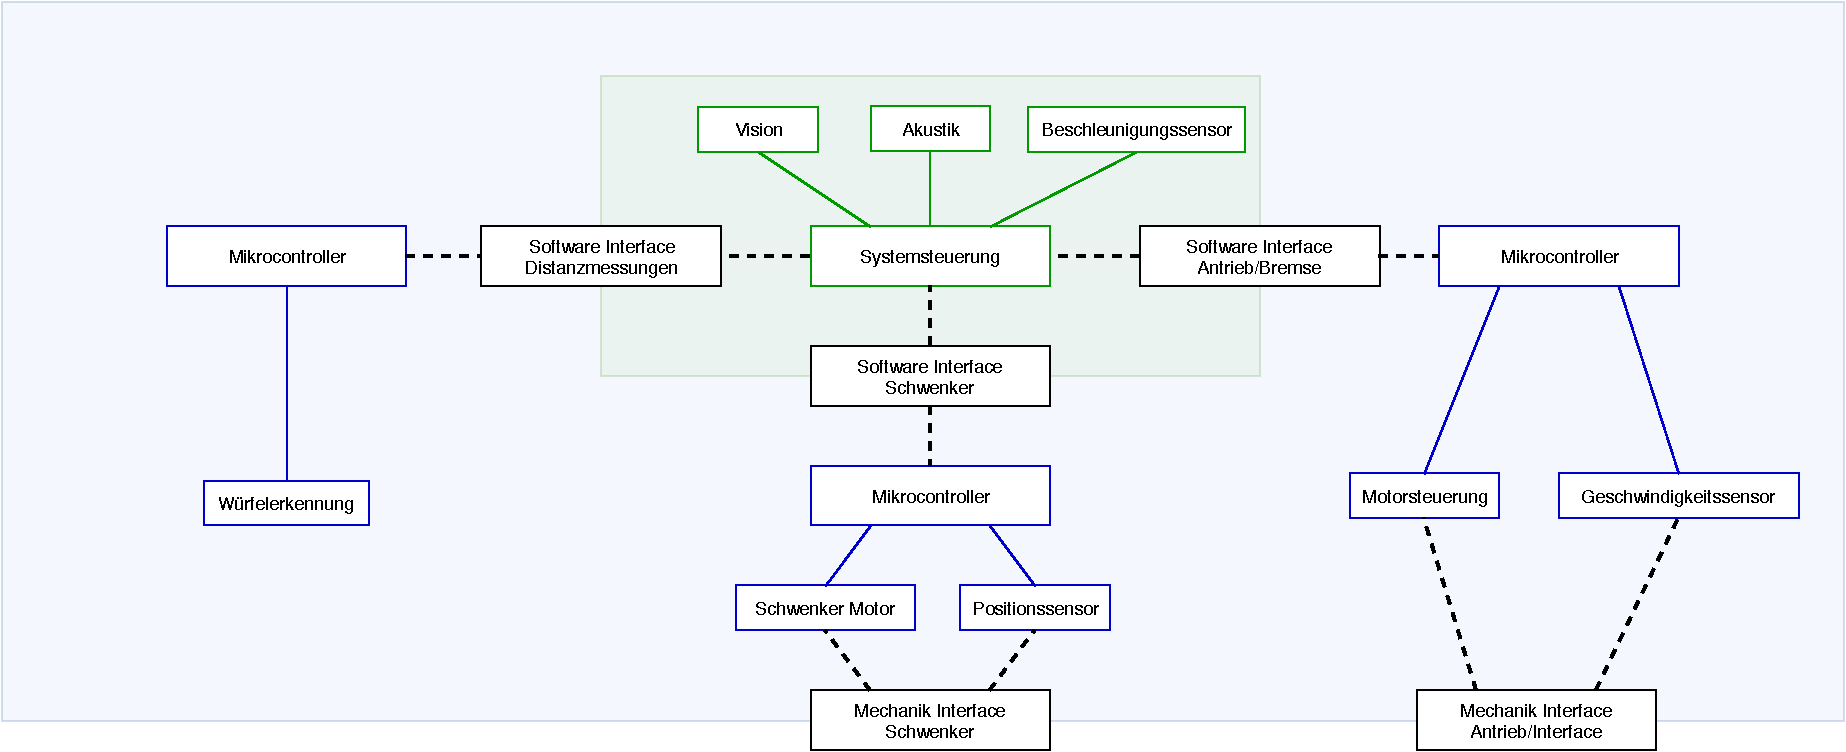
\includegraphics[width=1.0\textwidth]{../../images/Komponentendiagramm/Komponentendiagramm.pdf}
    \caption {Komponentendiagramm allgemein}
    \label{fig:komponenten_allg}
\end{figure}

\end{document}